\setlength{\columnsep}{3pt}
\begin{flushleft}
	\begin{itemize}
		\item The \textbf{"|"} character is pipe operator.
		\item A pipe is a technique for passing output of one command to another command:
		\bigskip
		\bigskip
		\begin{figure}[h!]
			\centering
			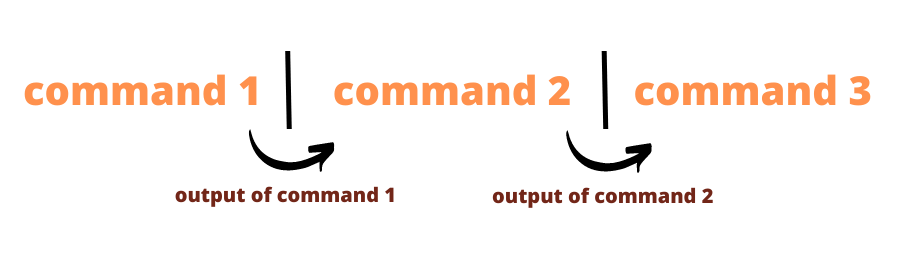
\includegraphics[scale=0.5]{content/chapter7/images/pipe.png}
			\caption{Pipe operator}
			\label{fig:pipe_operator}
		\end{figure}

		\bigskip
		\begin{tcolorbox}[breakable,notitle,boxrule=0pt,colback=pink,colframe=pink]
			\color{black}
			\fontdimen2\font=1em
			Syntax: command1 | command2 | command3
			\fontdimen2\font=4pt
		\end{tcolorbox}
	
		Eg: 
		\bigskip
		\begin{tcolorbox}[breakable,notitle,boxrule=-0pt,colback=black,colframe=black]
			\color{green}
			\fontdimen2\font=1em
			\# who | wc -l 			\color{yellow}#[press Enter]
			\newline
			\color{white}
			4
			\fontdimen2\font=4pt
		\end{tcolorbox}
		
		
	\end{itemize}
	
	
	
\end{flushleft}

\newpage

